\documentclass[hidelinks,12pt,dvipsnames,border=2pt]{standalone}
%\usepackage[top=0.7in, bottom=0.8in, left=1in, right=1in]{geometry}
\usepackage{tikz}
\usepackage{hyperref}
\usetikzlibrary{arrows}
\usetikzlibrary{shapes}
\usepackage{enumitem}
\usepackage{bm}
\usepackage{mathdots}
\usepackage{amsmath}
\usepackage{tcolorbox}
\usetikzlibrary{shadings}
\usetikzlibrary{decorations.pathreplacing}
\usepackage{helvet}
\usepackage{url}
\usepackage{graphicx}
\usetikzlibrary{arrows.meta,positioning,fit,calc}
\renewcommand{\familydefault}{\sfdefault}


\usetikzlibrary{arrows,decorations.pathmorphing,backgrounds,fit,positioning,shapes.symbols,chains}

\begin{document}
	
% trim=left botm right top
\begin{tikzpicture}

% manhattan
\node at (0,0) {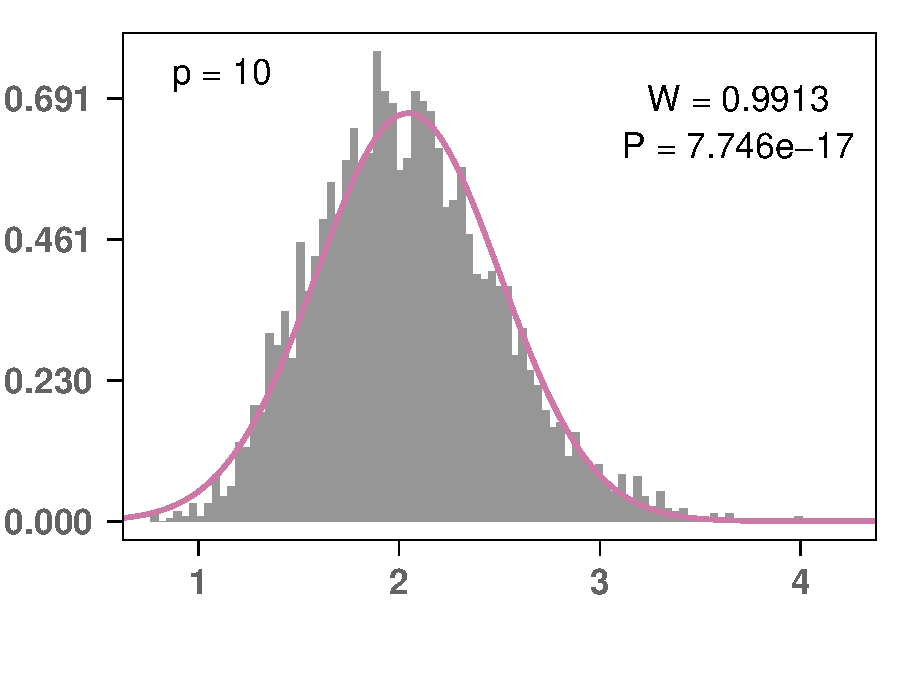
\includegraphics[width=\textwidth]{manhattan_histogram_p10.pdf}};
\node at (0,-9.2) {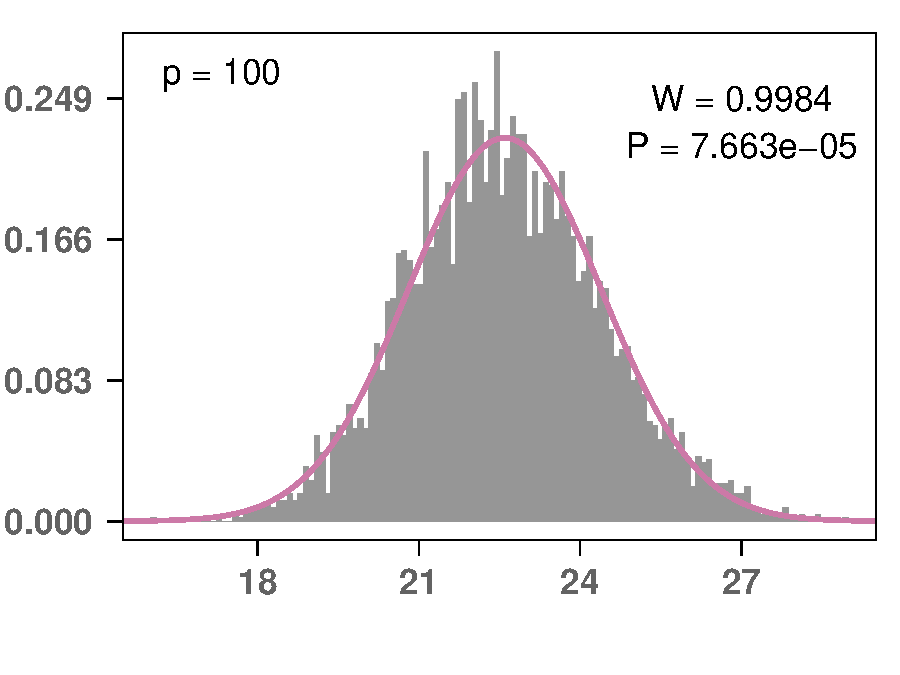
\includegraphics[width=\textwidth]{manhattan_histogram_p100.pdf}};
\node at (0,-18.4) {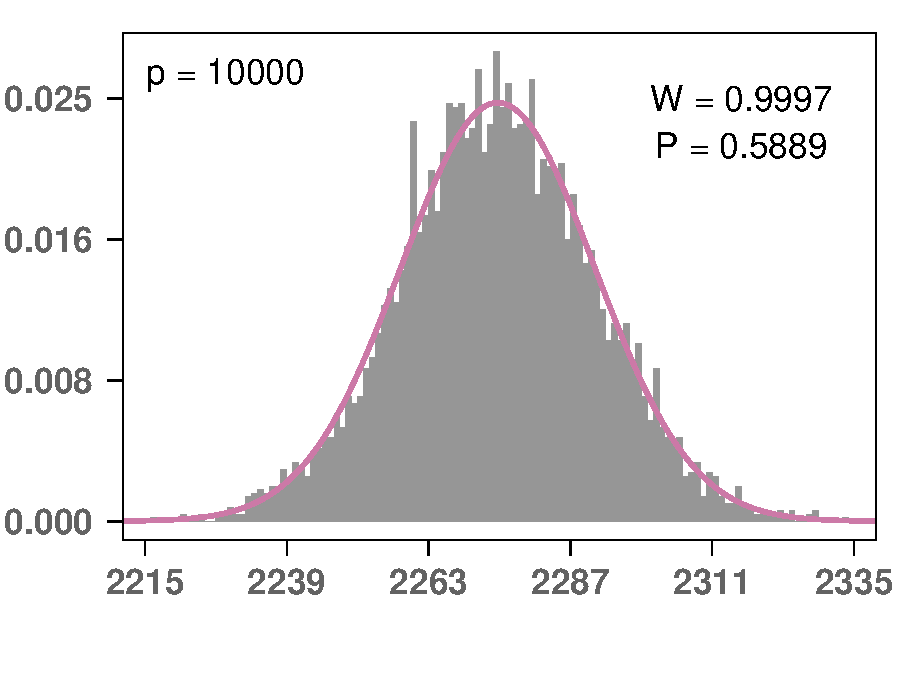
\includegraphics[width=\textwidth]{manhattan_histogram_p10000.pdf}};

% euclidean
\node at (14,0) {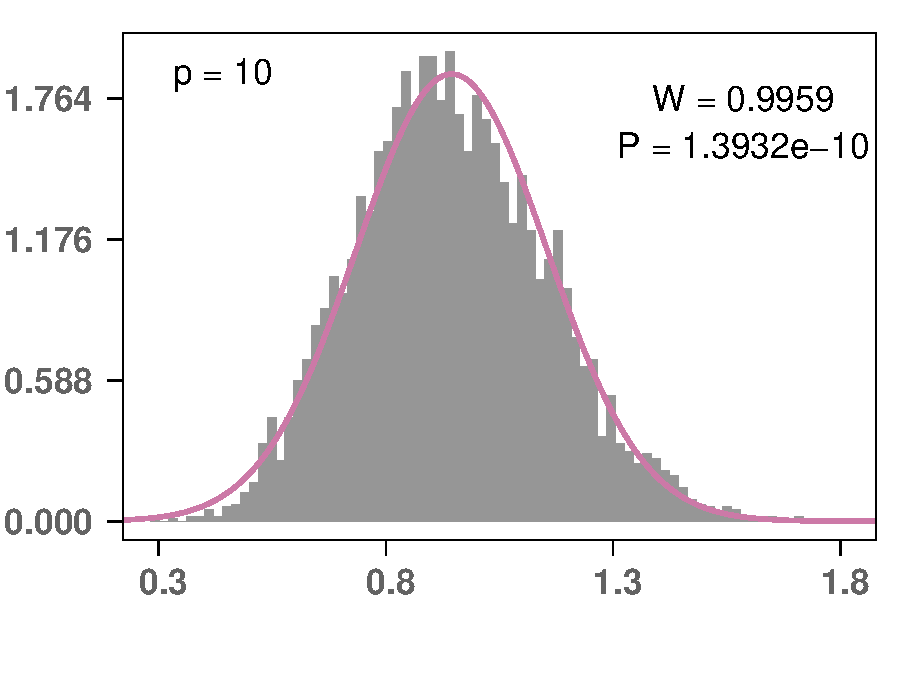
\includegraphics[width=\textwidth]{euclidean_histogram_p10.pdf}};
\node at (14,-9.2) {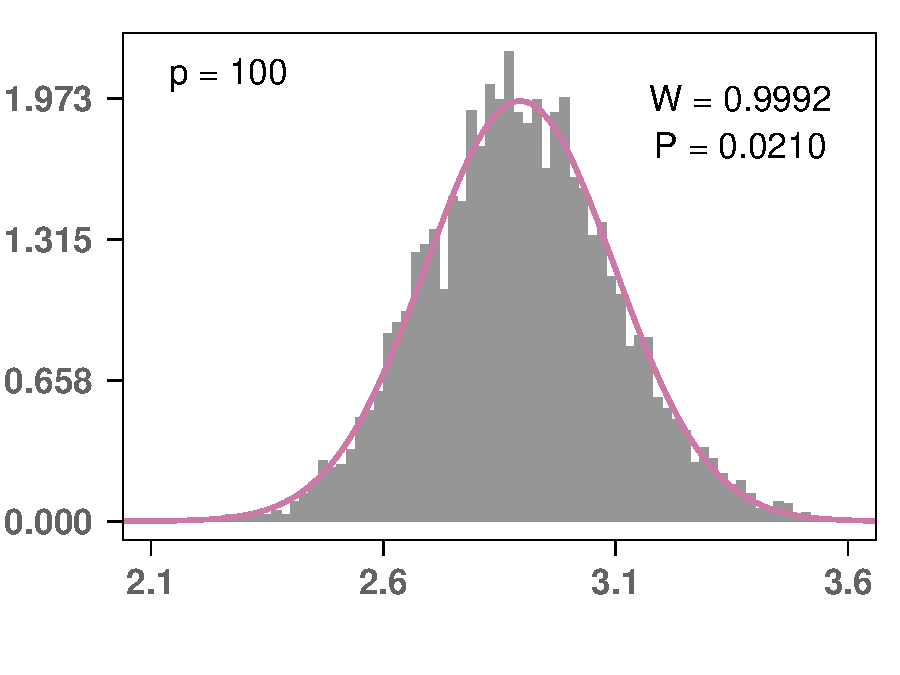
\includegraphics[width=\textwidth]{euclidean_histogram_p100.pdf}};
\node at (14,-18.4) {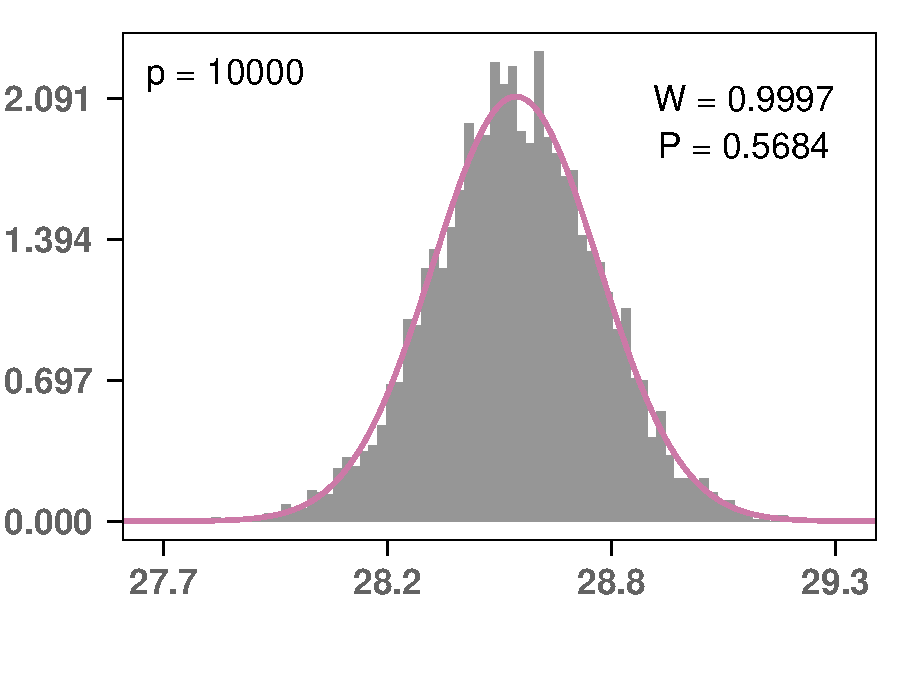
\includegraphics[width=\textwidth]{euclidean_histogram_p10000.pdf}};

% y label
\node[rotate=90,xscale=2,yscale=2] at (-7.7,-8.7) {Density};

% x label
\node[xscale=2,yscale=2] at (7.75,-23.2) {Distances};

% manhattan label
\node[xscale=2,yscale=2] at (0.75,5.5) {Manhattan};

% euclidean label
\node[xscale=2,yscale=2] at (14.75,5.5) {Euclidean};

\end{tikzpicture}

\end{document}